%iffalse
\let\negmedspace\undefined
\let\negthickspace\undefined
\documentclass[journal,12pt,twocolumn]{IEEEtran}
\usepackage{cite}
\usepackage{amsmath,amssymb,amsfonts}
\usepackage{graphicx}
\usepackage{textcomp}
\usepackage{xcolor}
\usepackage{txfonts}
\usepackage{listings}
\usepackage{enumitem}
\usepackage{mathtools}
\usepackage{gensymb}
\usepackage{comment}
\usepackage[breaklinks=true]{hyperref}
\usepackage{tkz-euclide} 
\usepackage{listings}
\usepackage{gvv}                                        
\def\inputGnumericTable{}                                 
\usepackage[latin1]{inputenc}                                
\usepackage{color}                                            
\usepackage{array}                                            
\usepackage{longtable}                                       
\usepackage{calc}                                             
\usepackage{multirow}                                         
\usepackage{hhline}                                           
\usepackage{ifthen}                                           
\usepackage{lscape}
\usepackage[export]{adjustbox}

\newtheorem{theorem}{Theorem}[section]
\newtheorem{problem}{Problem}
\newtheorem{proposition}{Proposition}[section]
\newtheorem{lemma}{Lemma}[section]
\newtheorem{corollary}[theorem]{Corollary}
\newtheorem{example}{Example}[section]
\newtheorem{definition}[problem]{Definition}
\newcommand{\BEQA}{\begin{eqnarray}}
\newcommand{\EEQA}{\end{eqnarray}}
\newcommand{\define}{\stackrel{\triangle}{=}}
\newtheorem{rem}{Remark}

\begin{document}
\parindent 0px
\bibliographystyle{IEEEtran}

\vspace{3cm}

\title{}
\author{EE23BTECH11217 - Prajwal M$^{*}$
}
\maketitle
\newpage
\bigskip

\renewcommand{\thefigure}{\theenumi}
\renewcommand{\thetable}{\theenumi}

\section*{Exercise 9.5}
\noindent25) \hspace{2pt} \textbf{Find the sum of the following series up to n terms and obtain the Z-transform:}
$$ 
\ldots + 0 + \frac{1^3}{1} + \frac{1^3 + 2^3}{1 + 3} + \frac{1^3 + 2^3 + 3^3}{1 + 3 + 5} + \ldots$$

\noindent Solution: 
\begin{align}
    x(n) & = \frac{\sum_{i=0}^{n} (i+1)^3}{\sum_{j=0}^{n} (2j+1)} u(n)  \\
    % & = \dfrac{\left(\frac{(n+1)(n + 2)}{2}\right)^2 }{(n+1)^2} \\
    & = \frac{(n + 2)^2}{4} u(n) \label{x(n)}\\\notag\\
    S(n) & = \sum_{r=-\infty}^{n} x(r)\\
    \notag \text{using \eqref{x(n)}, } \\
    & = \sum_{r=-\infty}^{n} \frac{(r+2)^2}{4} u(r) \\
    & = \sum_{r=0}^{n}\frac{r^2 + 4r + 4}{4} \\
    & = 1 + \frac{37n}{24} + \frac{5n^2}{8} + \frac{n^3}{12}
\end{align}

\begin{figure}[h]
   \centering
   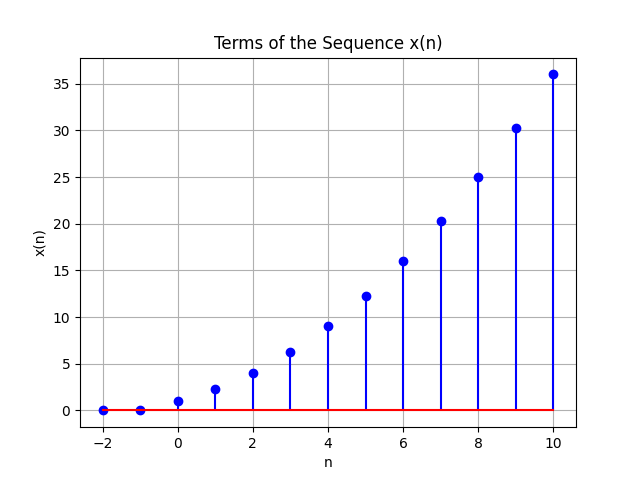
\includegraphics[width=1\columnwidth]{figs/plot.png}
   \caption{Plot of x(n) vs n}
   \label {fig: 11.9.5.25.1}
\end{figure}

\begin{align}
    x \brak{n} & \system{Z} X \brak{z} \\
    X \brak{z} = &  \sum_{n=-\infty}^{\infty} x \brak{n}   z^{-n} \\
    \notag \text{using \eqref{x(n)}, } \\
    = & \sum_{n=-\infty}^{\infty} \frac{(n + 2)^2}{4}u(n) z^{-n} \\
    = & \sum_{n=0}^{\infty} \frac{(n + 2)^2}{4} z^{-n} \\
    = & \sum_{n=0}^{\infty} \frac{n^2}{4}z^{-n} + \sum_{n=0}^{\infty} nz^{-n} \\
    & + \sum_{n=0}^{\infty} z^{-n} \notag\\ %remove notag and '\\ &' before submitting
    = & \frac{z(4z^2 - 3z + 1)}{4(z - 1)^3} & \cbrak{z\in\mathbb{C} : |z|>1}
\end{align}
\begin{table}[h]
    \centering
    
\begin{table}[h]
  \centering
  \begin{tabular}{|c|c|}
    \hline
    	\textbf{Symbol} & \textbf{Parameters} \\
    \hline
	  x(n) & general term of the series \\
    \hline
	  $X$(z) & Z-transform of x(n) \\
    \hline 
	  u(n) & unit step function \\
    \hline
  \end{tabular}
  \vspace{0.3cm}
  \caption{Parameters}
  \label{tab:parameters}
\end{table}

    \caption{Parameters}
    \label{tab: 11.9.5.25.1}
\end{table}

\end{document}

